Para atingir o objetivo deste artigo, criou-se uma Rede de Petri para simular um cruzamento com quatro semáforos.
A ferramenta CPN IDE foi utilizada para criar e simular a Rede de Petri~\cite{cpn-ide}.
Cada semáforo apresenta três estados possíveis: fechado (indicado pela cor vermelha), próximo ao fechamento (indicado pela cor amarela) e aberto (indicado pela cor verde).
Os semáforos foram dispostos, com dois na direção horizontal e outros dois na direção vertical.

A Figura~\ref{fig:traffic_light} apresenta a modelagem de um semáforo por meio de uma Rede Colorida de Petri.
Nesse modelo, cada lugar representa um dos estados possíveis do semáforo: fechado, próximo ao fechamento e aberto.
Todos os lugares são do tipo INT\@.
Inicialmente, cada semáforo inicia com duas fichas no estado fechado.
Três transições foram definidas: uma que move uma ficha do lugar vermelho para o verde, outra que move uma ficha do verde para o amarelo e, por último, uma que move uma ficha do amarelo para o vermelho.
Os arcos sempre consomem duas fichas.

\clearpage

\begin{figure}[ht]
	\centering
	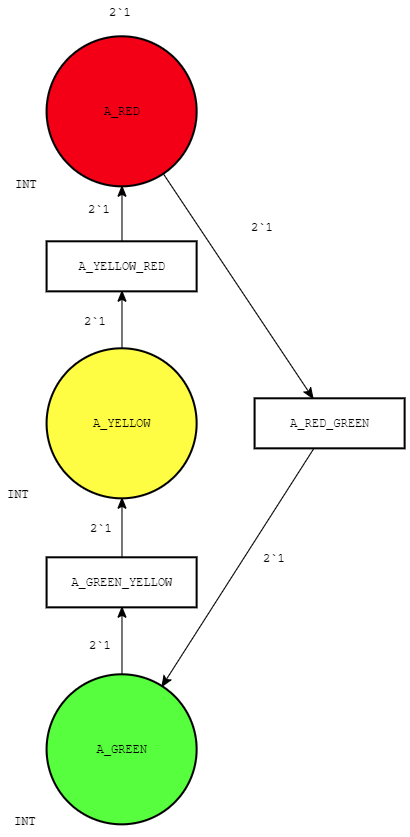
\includegraphics[width=0.55\textwidth]{images/traffic_light.png}
	\caption{Modelagem de um semáforo utilizando uma Rede Colorida de Petri}
    \label{fig:traffic_light}
\end{figure}

Para integrar-se com outros semáforos, foi necessário realizar algumas modificações na rede.
A Figura~\ref{fig:two_traffic_lights} ilustra a modelagem de uma Rede Colorida de Petri que conecta o funcionamento de dois semáforos.
Embora o semáforo em si permaneça inalterado, foram introduzidos novos arcos que vinculam os dois semáforos.

Dois arcos adicionais foram incorporados, consumindo fichas dos lugares vermelhos quando as transições de cada semáforo são acionadas, movendo a ficha do lugar vermelho para o lugar verde no mesmo semáforo.

Adicionalmente, outros dois novos arcos foram introduzidos, inserindo novamente fichas nos lugares vermelhos de cada semáforo no momento em que a transição que move a ficha do lugar amarelo para o lugar vermelho no mesmo semáforo é acionada.

Quando um dos semáforos está no estado aberto, os demais semáforos na rede devem permanecer no estado fechado, com as transições que alteram seus estados desabilitadas.
Os arcos que consomem fichas dos lugares vermelhos consomem apenas uma ficha, assegurando que o lugar vermelho do semáforo mantenha uma ficha, indicando assim o estado fechado.

Quando o semáforo que estava aberto retorna ao estado fechado, as fichas que foram consumidas dos outros semáforos devem ser restituídas.
Dessa forma, o arco que insere fichas nos lugares vermelhos dos semáforos passa a inserir apenas uma ficha, fazendo com que o lugar vermelho do semáforo volte a ter duas fichas, também indicando o estado fechado.

\begin{figure}[ht]
	\centering
	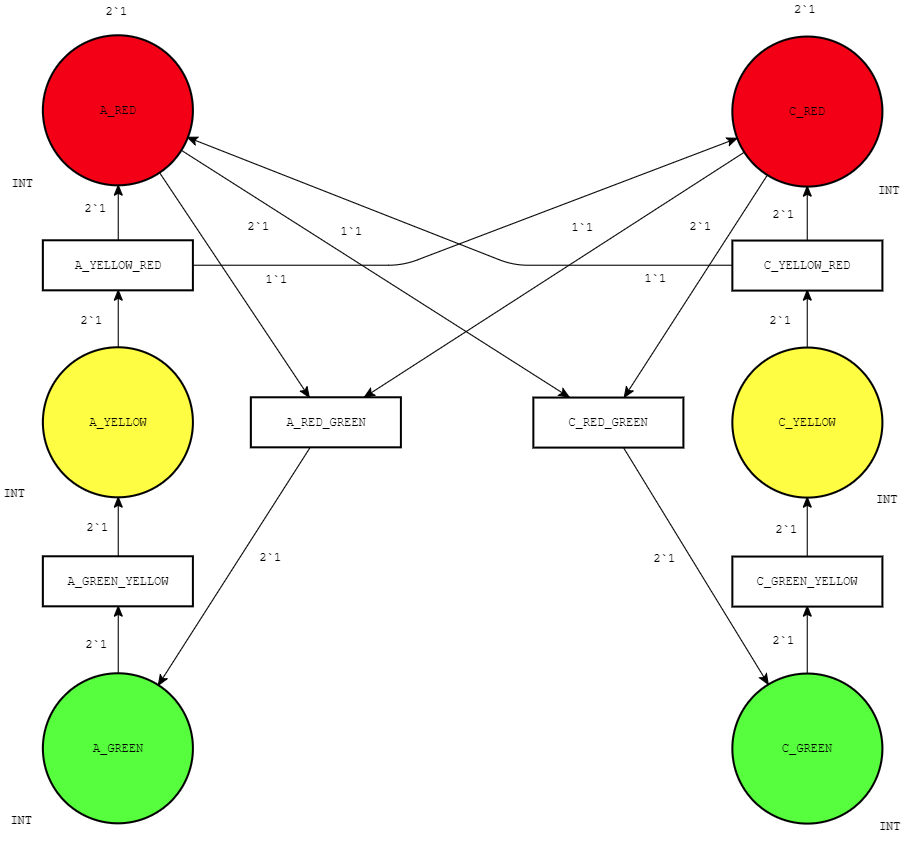
\includegraphics[width=1\textwidth]{images/two_traffic_lights.png}
	\caption{Modelagem da integração de dois semáforos}
    \label{fig:two_traffic_lights}
\end{figure}

Executando as adições correspondentes em cada um dos quatro semáforos, alcançamos a configuração final de nossa rede.
Nesse ponto, ocorre a movimentação consistente de fichas entre todos os semáforos, bem como a sua reposição.
A representação completa desse processo é visualizada na Figura~\ref{fig:full_petri_net}.

\begin{figure}[ht]
	\centering
	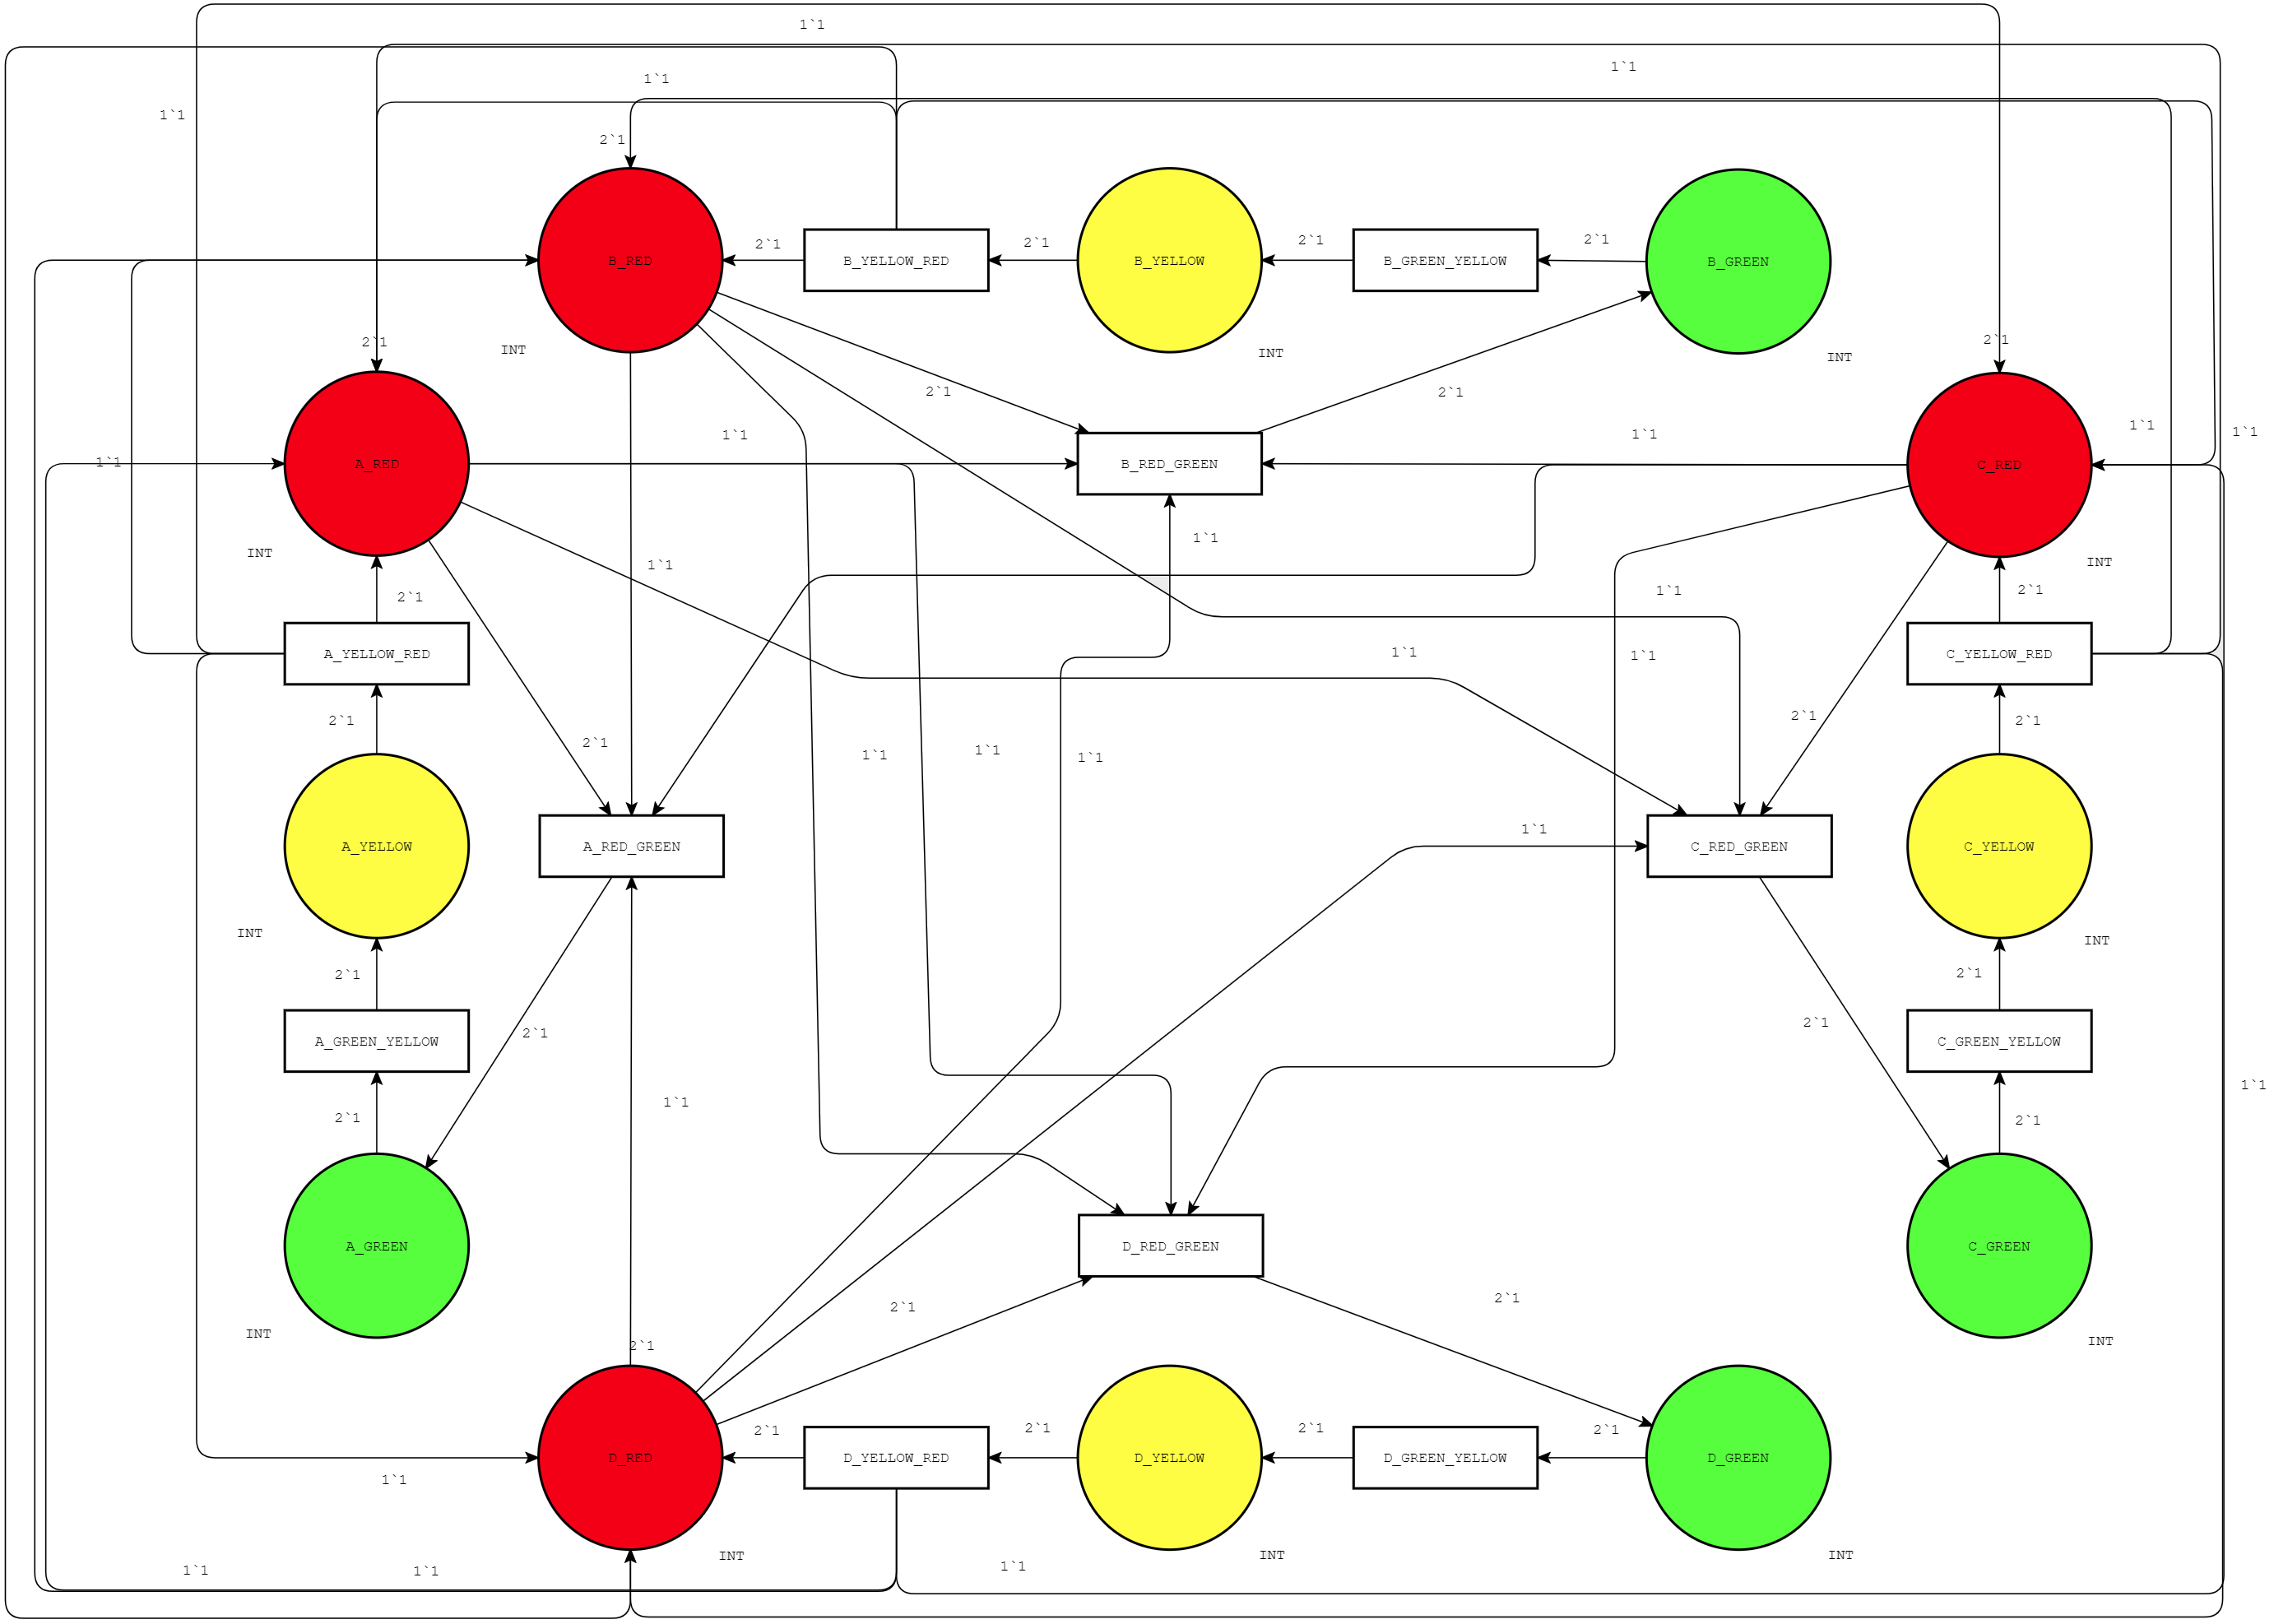
\includegraphics[width=1\textwidth]{images/full_petri_net.png}
	\caption{Modelagem completa do cruzamento de semáforos}
    \label{fig:full_petri_net}
\end{figure}